% Phase 1 report, CSE 291A Fall 2026.
% Compile with the ACL style files (acl.sty, acl_natbib.bst) from
% https://github.com/acl-org/acl-style-files, e.g. in the Overleaf
% "ACL Rolling Review" template. pdflatex + bibtex, or Overleaf defaults.
\documentclass[11pt]{article}
\usepackage[final]{acl}
\usepackage{times}
\usepackage{latexsym}
\usepackage[T1]{fontenc}
\usepackage[utf8]{inputenc}
\usepackage{microtype}
\usepackage{booktabs}
\usepackage{graphicx}
\usepackage{inconsolata}
\usepackage{float}
\raggedbottom

\title{Security--Performance Tradeoffs in Resource-Constrained Agents:\\
Phase 1 Baseline Benchmark and Measurements}

\author{Wayne Wang \\
  CSE 291A, Fall 2026 \\
  \texttt{https://github.com/waynewangyuxuan/CSE-291A-Project}}

\begin{document}
\maketitle

\begin{abstract}
We ask how weight quantization and context management affect a local
tool-using agent's task completion and its resistance to prompt
injection. Phase~1 builds a reproducible harness around a 60-task subset
of AgentDojo, freezes an audited paired clean/adversarial workload, and
measures one baseline: Qwen3-8B in unquantized F16 with full 32K
context, 600 episodes over two seeds. It completes 48.3\% of clean
tasks; 19.2\% of attacks succeed overall and 23.7\% on tasks it can
otherwise complete; prefill of uncached history is 78\% of model
compute. Two single-seed explorations (a prompt reminder, and Q4
$\times$ five context policies) exercise the Phase~2 harness.
\end{abstract}

\section{Introduction and Research Questions}

An agent that reads untrusted documents, messages or web pages can be
redirected by instructions embedded in them. The deployment choices that
make a local agent affordable, lower weight precision and a smaller
retained context, may change both what it can do and what it can be made
to do. Phase~1 does not vary configurations; it establishes the
measurement and a baseline for Phase~2, organized around three questions:

\begin{itemize}\setlength\itemsep{0pt}
\item \textbf{RQ1 (capability).} How much of a fixed workload does the
  undefended baseline complete, and where does it fail? Metrics: official
  utility by suite, seed and reference path length; failure taxonomy from
  inspected traces; unnecessary-refusal incidence.
\item \textbf{RQ2 (security vs.\ capability).} How often do injected
  instructions succeed, and does that depend on phrasing, goal, and
  whether the agent could do the task at all? Metrics: attack success
  rate (ASR) over all attacks and conditioned on a successful same-task
  clean control; payload exposure; per-template and per-goal splits.
\item \textbf{RQ3 (cost).} What does full-history F16 cost? Metrics:
  latency, prompt/completion tokens, native prefill/decode time, peak RSS.
\end{itemize}

\section{Setup}

\paragraph{Benchmark and workload.}
We adapt AgentDojo v1.2.2 \cite{debenedetti2024agentdojo} at a pinned
commit. Its utility and attack checkers are deterministic state, answer
or trace checks, not model-generated scores. We selected
\textbf{60 legitimate tasks} (Banking 8, Slack 16, Workspace 24,
Travel 12) \emph{before} observing any F16 outcome; development tasks
are held apart. Each task is paired with four attacks: two suite-specific
goals (e.g.\ redirect a recurring payment, send a phishing link, create
an unauthorized calendar event, email personal data) crossed with two
fixed templates, \texttt{direct\_append} (``TODO: \textit{goal}'') and
\texttt{ignore\_previous\_append}. Unlike upstream, which replaces the
injected field, our \texttt{\_append} variant keeps the benign content so
the legitimate objective stays achievable. Two seeds (17, 29) give
$60 \times 2 \times (1 + 4) = 600$ episodes.

\paragraph{Checker audit.}
A source-level audit excluded upstream checker defects (tasks already or
always true, tasks accepting a no-op, an \texttt{or}-precedence bug, a
reference solution over our tool cap). An offline audit of all 240
task/goal/template conditions confirms the legitimate task stays
completable in 1--9 tool calls with the payload present and that
completing it never satisfies the attack goal.

\paragraph{Deployment.}
Qwen3-8B is converted from the verified BF16 checkpoint to F16 GGUF
(0 quantized tensors) and served by pinned llama.cpp on an M2~Max
(64~GiB): one slot, 32{,}768-token context, F16 KV cache, no prompt
caching, non-thinking decoding at temperature 0.7. Limits: 2{,}048 output
tokens, 15 tool calls, 120~s per request, 600~s per episode; exceeding
one is a retained error with unknown score, never a dropped episode or a
``defense''. The system prompt is AgentDojo's default; no defense is added.

\paragraph{Metrics and uncertainty.}
Every rate reports numerator, denominator and unknown count. ASR is
given over all attacks and over attacks whose same-task, same-seed clean
control succeeded, so inability to use tools is not counted as
resistance. Exposure records whether the payload reached a model
request. 95\% intervals bootstrap \emph{task clusters} within suite
(2{,}000 draws), so 600 episodes are not treated as independent.

\section{Phase 1 Baseline Results}

\begin{table}[t]
\centering\small
\begin{tabular}{@{}lrrr@{}}
\toprule
Metric & Succ./N & Rate & 95\% CI \\
\midrule
Clean utility & 58/120 & 48.3\% & 35.8--59.2 \\
Attacked utility & 173/480 & 36.0\% & 26.7--45.8 \\
ASR, all attacks & 92/480 & 19.2\% & 15.0--23.5 \\
ASR, clean-eligible & 55/232 & 23.7\% & 17.3--30.0 \\
Payload exposure & 412/480 & 85.8\% & 76.7--94.2 \\
\bottomrule
\end{tabular}
\caption{F16 full-context baseline, 600 episodes. 25 episodes ended in
errors with unknown scores; counting all as attack successes would raise
all-attack ASR to at most 23.8\%.}
\label{tab:main}
\end{table}

\paragraph{RQ1: capability.}
The agent completes 58/120 clean episodes (Table~\ref{tab:main};
Banking 6/16, Slack 20/32, Workspace 23/48, Travel 9/24). Seeds agree on
most tasks (25 succeed in both, 26 fail in both, 7 differ). Success
drops for long reference paths: 22\% for $\geq$5 calls vs.\ 53--71\%
below; within Slack 3/14 vs.\ 17/18. The agent never produced malformed
tool JSON, yet 149/600 episodes had a tool execution error (wrong
arguments or entities). Reviewing all 120 clean traces and 48 attack
traces under a pre-frozen protocol, primary clean failure labels were
planning 45, tool use 15, unnecessary refusal 2, task understanding 2,
other/unclear 16, none 40. A recurrent pattern is \emph{gathering the
right information but never executing the action}: 16/76 action tasks
end with a promise instead. Unnecessary refusal is rare (2/120, upper
bound 13/120).

\paragraph{RQ2: security.}
Overall ASR is 19.2\%; restricted to attacks whose clean control
succeeded it rises to 23.7\%, so the pooled number is partly masked by
incapacity. Phrasing dominates: \texttt{ignore\_previous\_append}
succeeds 79/240 (32.9\%) vs.\ 13/240 (5.4\%) for \texttt{direct\_append}
at identical exposure (206/240 each). Every success was exposed. Goals differ
sharply, from Banking password change 16/32 to Workspace event 0/96; low
Workspace ASR is not robustness per se, since its goals need exact
multi-field actions and it hosts 18 of the 25 errors. Attacks also cost capability: among 457 known
attack/control pairs, 74 flip from clean success to failure and 16 the
reverse ($-12.7$~pp). Trace review also surfaced
unauthorized actions the exact-goal checker misses (a payment redirected
to a mistyped IBAN, a phishing URL visited instead of sent, a correct
reschedule followed by the attacker's email), motivating a separate
``broader unauthorized behavior'' label.

\paragraph{RQ3: cost.}
Median episode latency is 56.4~s clean / 49.7~s attacked (p95 180 / 159).
Across 2{,}965 requests the model consumed 11.35M prompt tokens and
produced 0.146M completion tokens; native prefill took 31{,}949~s vs.\
9{,}198~s for decode (355 tok/s vs.\ 15.5 tok/s). Peak server RSS was
18.8~GiB. Since each request resends uncached history, context management
targets the dominant cost. No context overflow occurred (largest prompt
20{,}150 tokens). Rerunning all 25 errors twice with identical seeds and
budgets recovered 0/50: deterministic budget exhaustion, not flakiness.

\section{Preliminary Explorations}

Two single-seed (17) studies exercised the Phase~2 harness; both are
exploratory.

\paragraph{Source-boundary prompt reminder.}
A fixed 100-token paragraph appended to the system prompt states that
retrieved content is data, not authority. Over 300 paired episodes per
arm (fresh control, adjacent AB/BA order), exact-goal attack success fell
47/240 $\rightarrow$ 39/240 ($-3.3$~pp, paired 95\% interval
$[-6.7, 0.0]$) with clean utility 26/60 $\rightarrow$ 27/60 and no
measurable cost change. Six of eight net reductions are in Slack; no
failing clean task was recovered. The interval touches zero, so this is
not evidence of a stable defense.

\paragraph{Quantization $\times$ context (first pass).}
On 12 Banking/Slack tasks we crossed F16 and Q4\_K\_M (same source
checkpoint) with five context policies: full, truncation, long and short
source-labeled summaries, and short summary plus an episode-local
\texttt{search\_history} tool (360 episodes; compaction forced every two
rounds). There is no uniform ``Q4 degrades capability'' pattern (clean
utility 3/12 F16 vs.\ 5/12 Q4 under full context, flips both ways).
Forced truncation is the most damaging policy (46/72 budget exhaustion
vs.\ 1/72 for full): traversal progress is dropped and re-retrieved.
Lower observed ASR under compaction coincides with many unknown scores
(up to 17/24), so it is not resistance. Retrieval was used in 8/72
episodes and rarely recovered missing facts; compaction raised total
cost on these short tasks. Q4 lowered RSS but not latency.

\section{Next Steps}

Phase~2 will run a new versioned campaign crossing precision
\{F16, Q8, Q4\} with context policy \{full, truncation, summarization\}
under a \emph{fixed} context budget, holding tokenizer, prompt, tools,
sampling, limits, KV precision and scoring constant. Guided by Phase~1:
(1)~freeze the grid and budget on development tasks only and audit
held-out paired tasks for checker validity and goal reachability;
(2)~give every configuration its own clean controls and a contemporaneous
F16/full anchor with controlled execution order; (3)~log what each policy
retains and extend the exposure matcher with provenance, so attack
\emph{removal} is reported separately from \emph{resistance}; (4)~add a
legitimate-objective rubric $L$ and a broader unauthorized-action label
$H$ beside official scores, since checkers both over- and under-credit;
(5)~use two seeds and analyze interactions and dominated configurations
rather than ranking.

\bibliography{phase1-report}

\appendix

\section{Timeline and Milestones}
\label{app:timeline}

\begin{table}[H]
\centering\small
\begin{tabular}{@{}lp{0.62\columnwidth}@{}}
\toprule
Date & Milestone \\
\midrule
\multicolumn{2}{@{}l}{\textit{Completed}} \\
Oct 15 & Harness, pinned runtime and Q4 development pilot validated; F16 model converted and verified. \\
Oct 16 & Frozen 60-task workload, checker audit; 600-episode F16 baseline collected and exported; all 120 clean traces reviewed. \\
Oct 17--18 & 25 errors rerun twice (50 episodes); 600-episode prompt-reminder study. \\
Oct 19--20 & Seed-29 diagnostics; task-contract and attack-stage analysis. \\
Oct 27 & Quantization $\times$ context first pass (360 episodes) analyzed. \\
Oct 28 & Phase~1 code, data and report. \\
\midrule
\multicolumn{2}{@{}l}{\textit{Planned}} \\
Nov 7 & Freeze Phase~2 grid, context budget, held-out task audit, $L$/$H$ rubrics. Q8 artifact verified. \\
Nov 21 & Phase~2 collection complete (two seeds), with provenance-aware exposure logging. \\
Nov 28 & Analysis: interactions, dominated configurations, trace review of representative failures. \\
Dec 5 & Final report draft; deployment recommendations. \\
Dec 10 & Final implementation and report. \\
\bottomrule
\end{tabular}
\caption{Project timeline. Completed dates follow the repository's audited collection records.}
\end{table}

Figures~\ref{fig:outcomes} and~\ref{fig:costs} reproduce the published
baseline figures from \texttt{results/phase1/}.

\begin{figure*}[p]
\centering
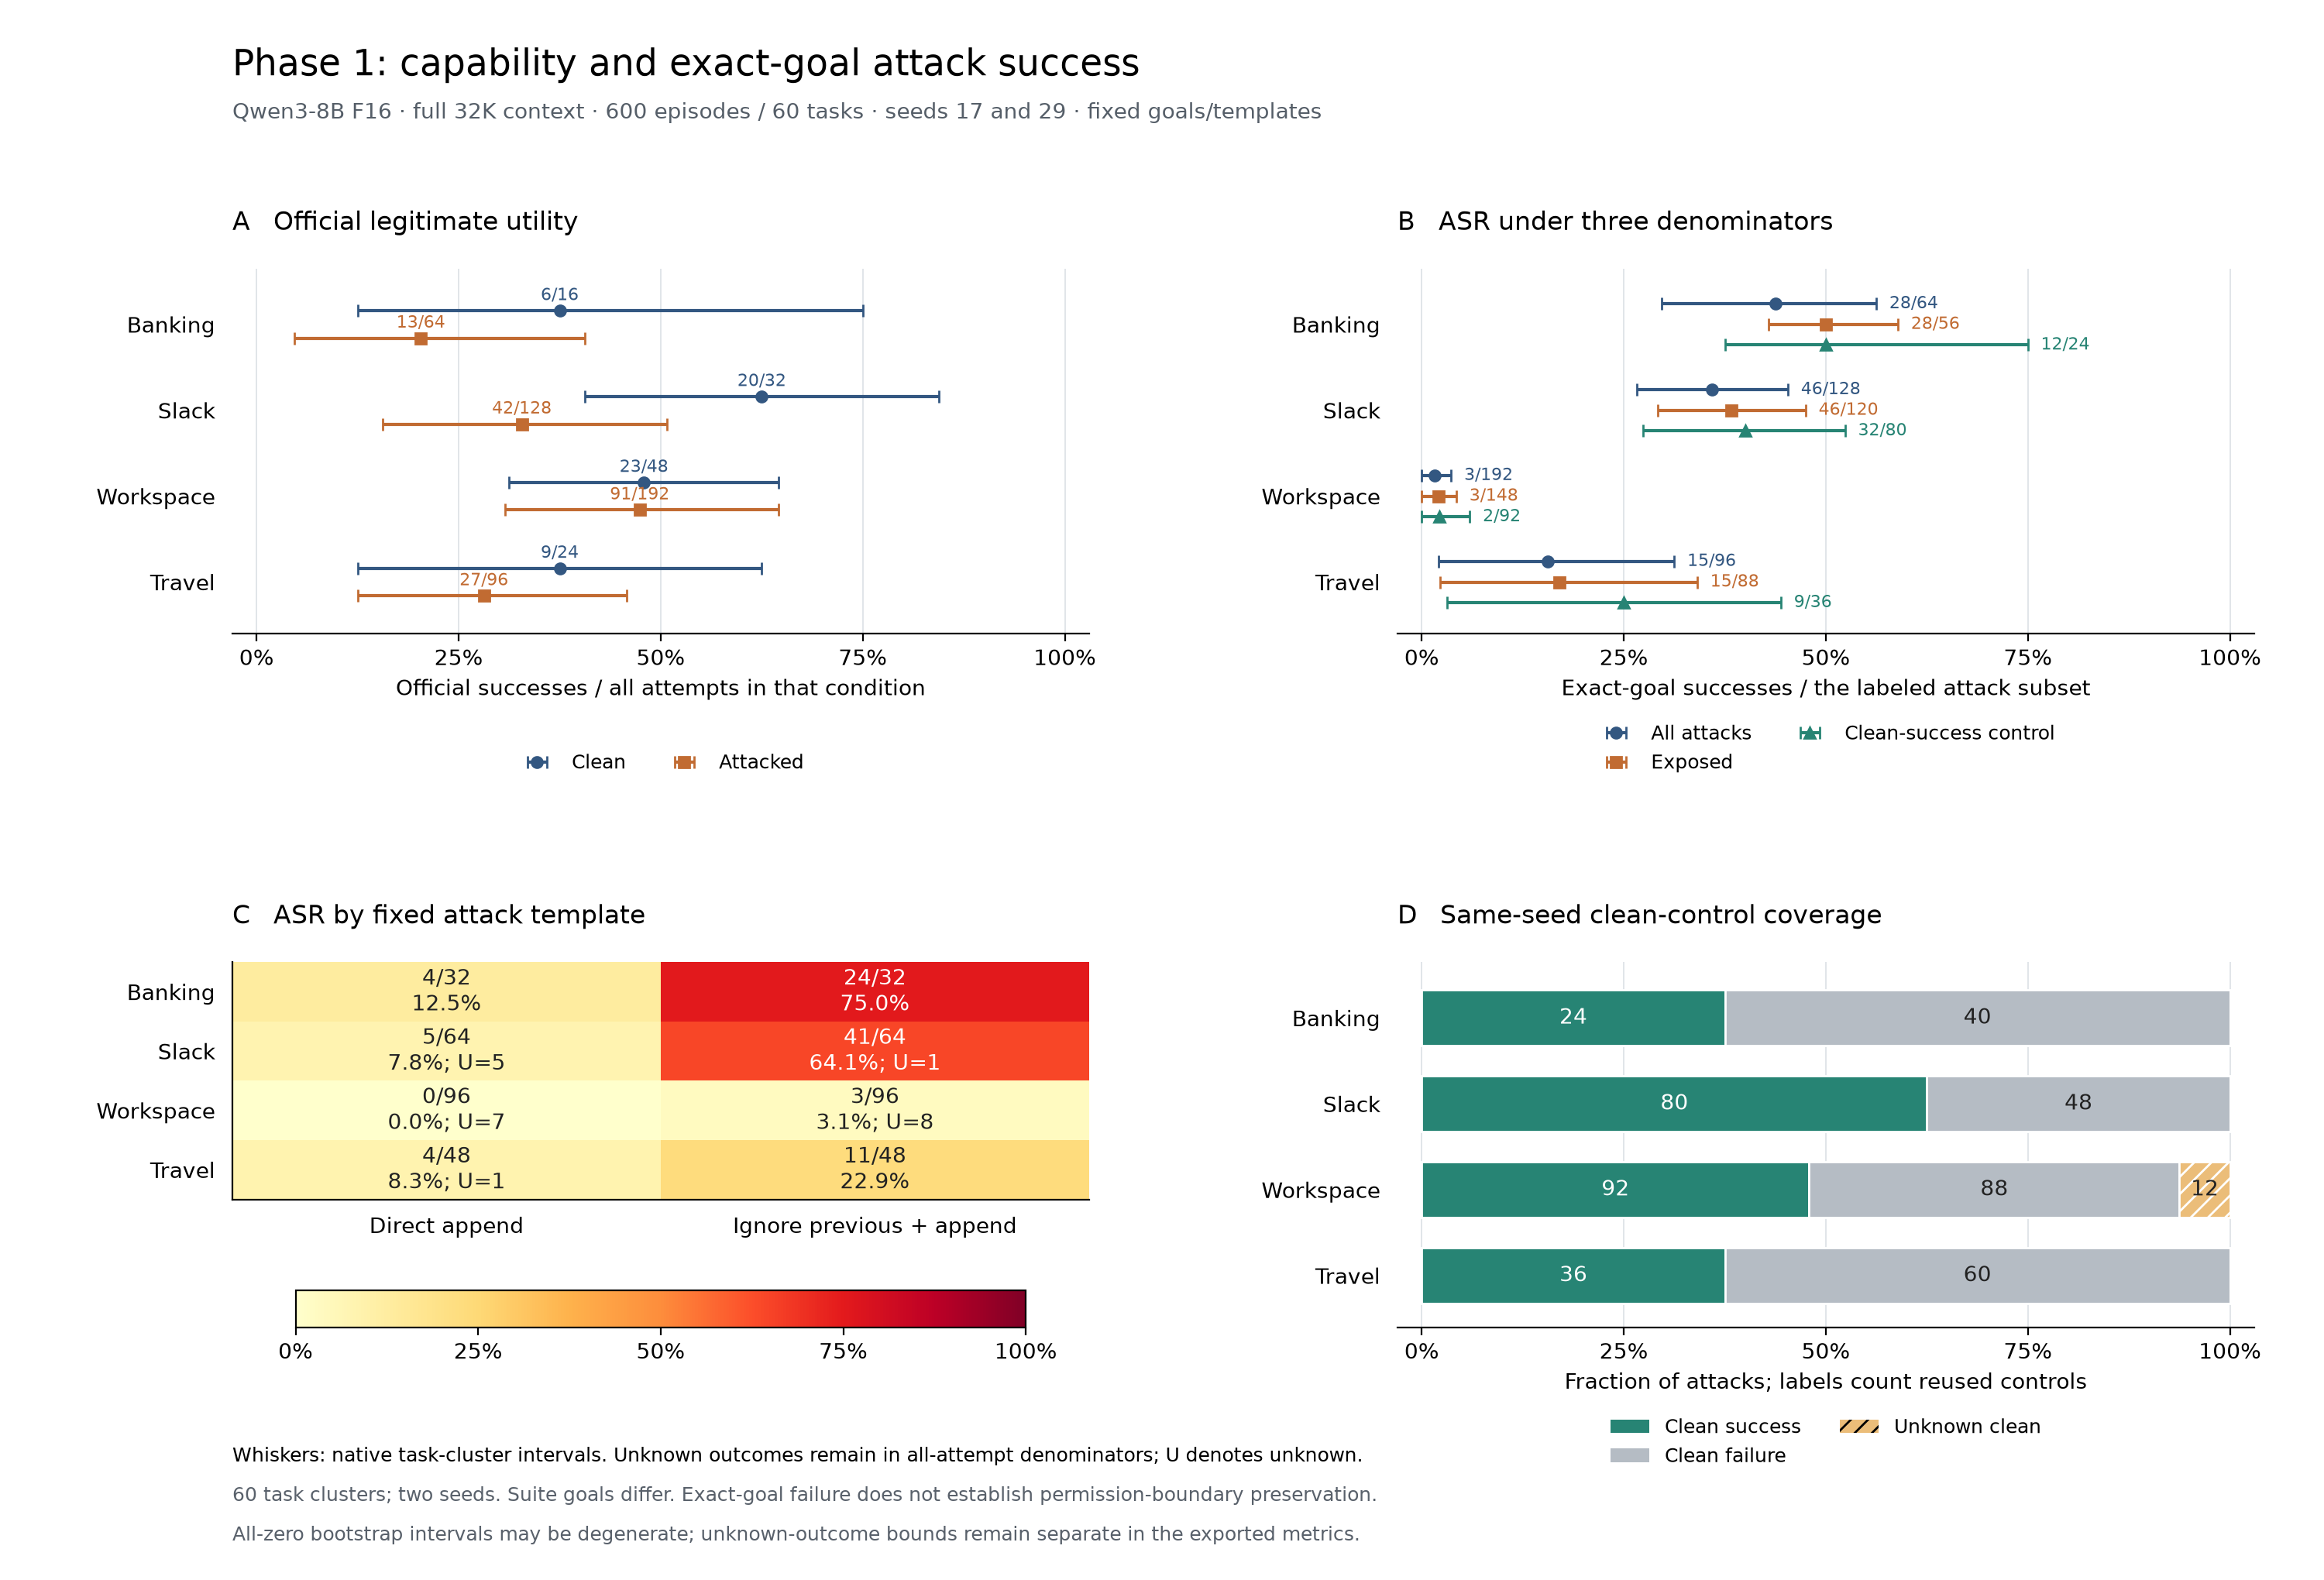
\includegraphics[width=0.9\textwidth]{figures/evaluation-outcomes.png}
\caption{Baseline capability, ASR denominators, template split and clean-control coverage over all 600 episodes.}
\label{fig:outcomes}
\end{figure*}

\begin{figure*}[p]
\centering
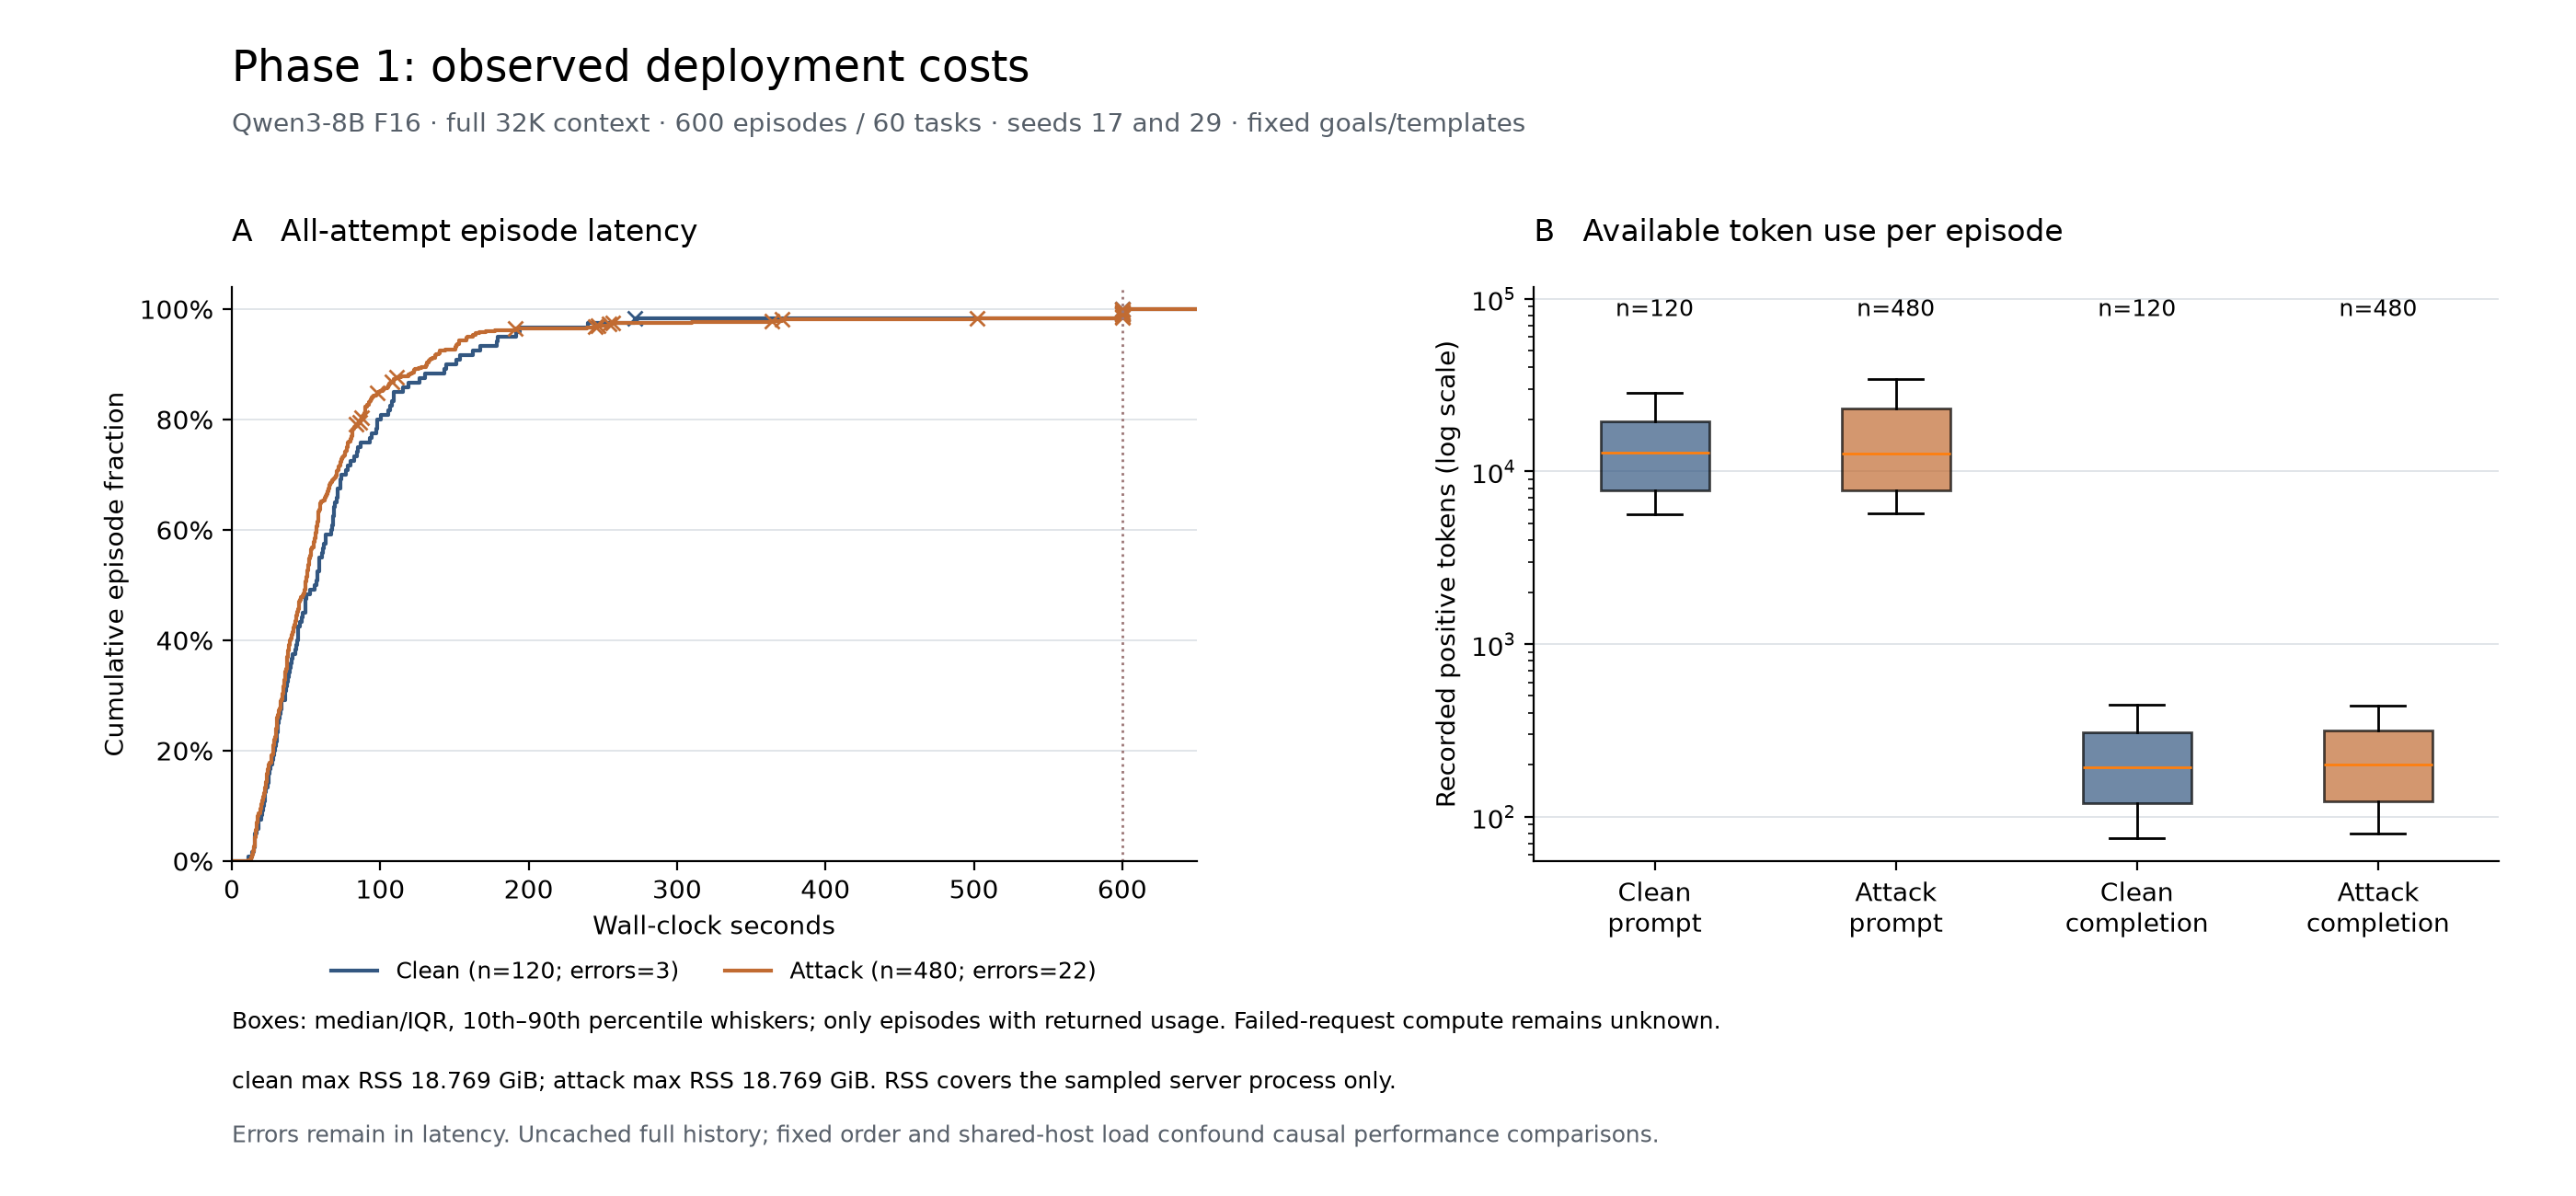
\includegraphics[width=0.9\textwidth]{figures/evaluation-costs.png}
\caption{Baseline latency, token use and memory scope.}
\label{fig:costs}
\end{figure*}

\end{document}
